
\chapter{Exploration 3 (part 3): assessing the benefits for porting XIMPEL to React}
\label{chap:exploration3}

% Leg de titel uit en waarom part 1 en 2 weg zijn
Why would a chapter start with part 3? There is of course only one sensible explanation: part 1 and part 2 -- also described as first attempt and second attempt -- have been kidnapped. On a more serious note, the relevant elements of part 1 and part 2 are in this chapter as well, but it is part 3 that presents how XIMPEL could be effectively and efficiently be ported to React. However, in an attempt to preserve how the exploration went, this chapter has been labeled part 3 and the other two parts are in the appendix.

% Leg uit waarom je voor ReactJS koos
With that said, ReactJS is hip, new and shiny. It introduces a relatively unknown paradigm to web developers called reactive programming. I wanted to work in this language because the web community seems to settle on this as a best practice method of creating web applications. Moreover, if my thesis supervisor can demand that I work on his framework pure for promotional reasons, then I can decide I learn a new framework for self promotional reasons. Later on I also justified the use of React academically but I do not want to shy away from the inherent selfishness that academia has. If science is a form of truth discovery, then the truth of its process should not be hidden.

Related to this is that I wanted to create the same type of exploration that Stefan Bruins did. If Stefan Bruins can port XIMPEL to JavaScript and call it academic, then I can do the same for porting the JavaScript version of XIMPEL to React. I believe in both cases the research question of ``is it possible?'' could be answered a priori with a ``yes.'' However, like Stefan I am an empiricist and the strongest form of evidence is through physical demonstration. Moreover, I altered the research focus to whether XIMPEL written in ReactJS (from now on called XIMPEL React) has more advantages than XIMPEL written in JavaScript + jQuery (from now on called XIMPEL JS). That answer is a lot tougher to answer a priori and hence an actual implementation, including a write up of the whole implementation experience is needed.

% I should tell here that XIMPEL has one powerful feature that React has as well: the ability to create components.
On another note, this started out as exploration 3, but part 3 of the exploration occurred later than exploration 4, 5 and 6. Therefore, it could also been seen as the final exploration. 

The reason this exploration started in the first place is because XIMPEL shares an idea that ReactJS has as well. They both have components. XIMPEL has it in the form of a playlist, where every component could be seen as a sort of invocation towards execution of the actual component. It is analogous to a function invocation and function definition. ReactJS is not bounded by a playlist, it has components everywhere; it also has the idea of component invocation and component definition, like XIMPEL. Figure \ref{images:architecture_playlist_to_component_mapping} shows this thought.

My questions specifically regarding this exploration are: is it possible to make use React and its ecosystem to port XIMPEL to React efficiently and effectively? Moreover, what are other possible benefits or disadvantages regarding this port? 


% glossary:
% media type: a specific media class name (e.g. Video or Audio) in both plain JS XIMPEL and XIMPEL React
% media item: a specific instance of any media type

% TO DO
% Short story exploration 3
% Discussie opnemen over welke features erin en welke niet -- justification
% Op welke manier passen questions in XIMPEL?
% React als ecosysteem? Te doen?
% Maintainability
% Is de React codebase zinvol? Voor? Tegen? Eventuele uitbreidingen?
% Duidelijk formaat exploratie. (geldt voor alle exploraties)
For porting XIMPEL to ReactJS I thought it had the following advantages:
\begin{itemize}
    \item A lot of parsing logic could be done via ReactJS and Webpack by transforming the XIMPEL playlist to a declarative language that is completely compliant with JSX. So there is no need to create a parser.
    \item The virtual DOM would replace the in-memory configuration code that has been written for XIMPEL. So there is no need to write in-memory configuration code.
    \item Cross-browser support is suddenly managed by the maintainers of the ReactJS framework.
    \item By teaching XIMPEL to students, it is needed to teach about ReactJS to students who want to extend XIMPEL. This introduces them to some of computer science concepts implicitly.
\end{itemize}

% Veel parsing logic kan via React worden gedaan en hoeft niet meer worden opgeschreven, omdat de XIMPEL playlist basically een JSX datatype wordt.
% Hetzelfde geldt voor de playlist tree dat in het geheugen wordt opgeslagen: React doet dit via de virtual DOM.
% Het maken van mediatypes en dergelijke wordt ook een stuk flexibeler, omdat het aanmaken van een mediatype betekent dat er een extra React component wordt gemaakt.
% Nu kun je mensen stiekem HTML/CSS onderwijzen als ze een XIMPEL playlist maken, terwijl de kern van XIMPEL blijft bestaan. 

% Een mogelijk nadeel:
% Een nadeel is dat elke child node (HTML of React Component) onder elke child node mag waardoor er invalid playlists kunnen bestaan. React is misschien te expressief. Het nadeel is volgens mij niet heel groot, omdat de gebruiker er visueel mee wordt geconfronteerd.

In short, the idea was to see if it is possible to make the ReactJS framework work for us. If this is possible, then we as XIMPEL developers have a free lunch! Who does not want a free lunch?


% De voordelen 1 tot en met 3 blijken onwaar te zijn. Ik kwam erachter dat veel parsing logic en playlist tree logic nog steeds geprogrammeerd zou moeten worden, en het maken van eigen mediatypes zou net zo flexibel zijn -- niet flexibeler. Voordeel 4 is echter wel waar, mits je XML opgeeft en studenten laat programmeren in JSX, maar dan wordt XIMPEL ook wat complexer helaas. Mijn XIMPEL React programma laat wel zien hoe je XML kan vertalen naar React components, wat ik supergaaf vind om te zien! :)

To validate these assumptions I made a very simple prototype of creating a custom React component in an XML file. The XML file would be read in by a React class that I programmed. What I found is that this exploration failed so dramatically that for more than 6 months I believed to have invalidated most advantages. You can read a full write up of the failure in appendix \ref{chap:exploration3_appendix_part1}.

However, by writing the chapter 6 months later, I was forced to take a closer look at the source code. Because I needed to look at the source code, I needed to look at the dependencies. And when I looked at the dependencies, I noticed that the XML parser of Webpack uses a library in order to parse the XML. There seemed to be a small detail that I missed. Upon further inspection this dependency of the XML parser of Webpack showed that the XML parser was configurable! Unfortunately, I did not see this before. So I could do a lot more in my second attempt, which is described in the next section.

\section{Webpack XML parser setup}
There were two modifications that allowed for a much more successful exploration compared to the first time. First, I modified the parser to have an explicit tree structure by preserving order between siblings and parent-child relationships. In general, it is the question whether an XML document needs this type of order preserved since some XML documents could be treated as an unordered set. 

For XIMPEL, it is needed that the XML document would be parsed as an ordered array. This feature gives more power to the programmer, in the same sense that a Turing complete system has more computational power than a finite state machine. Without order there is chaos, and in this particular case there would sometimes be no way to determine which media item (such as a video or image) or subject should be loaded first.

The second modification helped a lot in code readability. While it is not as game changing or groundbreaking as the first, code readability is a necessary requirement for a fruitful collaboration on any software project. For example, the default setting to denote attributes of a parsed XML tag itself was `$`. To denote inner text it was `_`. And children was `$$`. I renamed this to: `attributes`, `text` and `children` respectively.

%TO DO: some bug is in here!
\section{Implementation methodology of the second and third attempt}
In the second attempt of this exploration I tried to explore if I could re-implement XIMPEL quickly since the possibility of it is one of the main questions. I did not consider architecture -- or even best practices for programming React. This has led to quite a bit of technical debt. Creating technical debt has also been done in order to find out what architectural patterns work and which does not. Another reason to create technical debt is because I follow the programming philosophy of Jonathan Blow, which is: try to produce as fast as possible and then when you hit performance bottlenecks or any other bottleneck of any kind, only then try to be smart about solving that bottleneck. In some of his YouTube videos he goes in-depth how the code that he created for his award winning games like Braid and The Witness only have 6 to 10 percent of optimized code
\footnote{I forgot which video, but here is his channel: \url{https://www.youtube.com/channel/UCCuoqzrsHlwv1YyPKLuMDUQ}.}. 
It has also been done in order to find in which regards one needs to fight the React framework and in which cases React gives the developer wings to fly and develop certain features of XIMPEL a lot faster.

This approach worked. However, while it worked it did create an issue too big to ignore when it came to infinitely nesting the `<media>` tag (which allows for parallel play and is presumed as default by giving it the `<media>` tag) and the `<sequence>` tag (which allows for sequential play). Since infinitely nesting parallel and sequential play is a feature essential to any hypermedia framework, I decided to revise the architecture and brush up a bit on the best practices of ReactJS. This also meant that I almost completely restarted from scratch, except for the Webpack XML parser setup, which is exactly the same. The inner workings of my second attempt is also put in the appendix which can be read in appendix \ref{chap:exploration3_appendix_part2}. Besides the necessity of revising the architecture and learning more about React's best principles, I still had the same programming philosophy in mind inspired by Jonathan Blow.

To summarize, there have been three attempts in porting XIMPEL to ReactJS. The first attempt did not go anywhere (see appendix \ref{chap:exploration3_appendix_part1}), the second attempt did but had an architectural flaw (see appendix \ref{chap:exploration3_appendix_part2}) and the third attempt has an architecture that is clear and one that works. The third attempt will be exclusively presented in the next sections  (without the first and second attempt). The final two attempts do have a couple of things in common (e.g. overlays, Webpack setup and data flow philosophy). So some paragraphs in the appendix are the same as they appear in the chapter here.

% Not everything has an error message
\section{Designing XIMPEL React}
While porting XIMPEL JS to XIMPEL React, I decided to leave some features out. I did this in the interest of time and in the interest of vision. The requirements of a fixed width and height 1920 by 1080 has been dropped. This is because there is more focus on displaying (hyper)media than XIMPEL being an interactive video player. The `<quiz>` tag has been left out since it can be modelled already through other language constructs that XIMPEL provides. One way to model it can be seen in figure \ref{tikz:full_graph}. The pause, stop and play functionality has been dropped, because I hypothesize that these features make users assume that time scrubbing is an available feature. The error message system has been altered as well. Tags that are not allowed are shown as an error message on the page, because not every XIMPEL author knows about the JavaScript console. Unknown attributes are not shown as an error message, it would be more productive to do so but experienced authors can find them quite quickly and inexperienced authors learn a thing or two about debugging. This is an educational experience that every XIMPEL author should be familiar with.

Every exploration that I wrote contributed at least a small feature to XIMPEL React, most of which are also in XIMPEL JS. The ability to play parallel media (exploration 2), integrate a terminal (exploration 1), log user data and capture their facial expressions (exploration 4), media items surviving a subject switch (MISSS, see exploration 6) and even simply leaving the time scrub bars in for audio and video (inspired by exploration 5, this feature is not in XIMPEL JS). 

The process of the design happened intuitively. The requirements of porting are quite clear and so is the problem definition regarding re-implementing XIMPEL. Normally, the first major step is devizing the architecture and I decided to program it iteratively. By programming an architecture iteratively, it is possible to see what works and what does not work in earlier versions of XIMPEL React. Furthermore, a lot of the design process also occurred by virtue of writing this thesis and revising this chapter more than any other chapter.

\section{Architecture}
% Also describe how you make the playlist a little bit smaller the whole time
In this section it is described how the third attempt improved upon the second attempt from an architectural standpoint, since improving and implementing the architecture is the biggest difference between the two attempts. Then, a small explanation of some terminology known in compiler construction will be added to our vocabulary in order to explain this architecture better. Then, the rules of all components are described. While it is not a comprehensive rule list it does give a good idea of what XIMPEL React is capable of on a per component basis. Describing rules on a per component basis does not give the full picture, which is done in the subsequent sections.

\subsection{Improvements compared to second attempt}
The general idea of the architecture is that each XML tag has its own component. This component is responsible for rendering its own level, which is an improvement compared to the second attempt where there was one top level component trying to render everything. For example, a media type like the `<image>` tag would render its own image via the HTML5 `<img ... >` tag. The `<sequence>` tag would render as a `<div ...>` in HTML5. Another improvement is regarding the in-memory configuration which is an object that is created by Webpack which parsed the XML file. In the second attempt, the in-memory configuration consisted of actual React elements. In the third attempt the program uses the parsed XML by Webpack as the in-memory configuration. This eliminated a whole host of introspection issues since React elements (2nd attempt) are tougher to inspect compared to an XML in-memory configuration (3rd attempt). One potential tried solution was to stringify React elements to JSON and do a string match. This did not work, because a React element has circular dependencies, which means the stringification to JSON will never complete. Contrast that to parsed XML which had a `#name` property which indicated the type of the parsed XIMPEL tag (e.g. `audio`\footnote{Indeed, it is with a lowercase `a`, React elements and components would be with an uppercase `A` but in XML form it is a lowercase `a`}). A third improvement is regarding the communication, which has been streamlined regarding the publish-subscribe communication pattern. Specifically there are fewer `publish(...)` and `subscribe(...)` calls.

% \incgraph[documentpaper,
%   overlay={\node[red] at (page.center) {\Huge Picture sized to paper};}]
%   [width=\paperwidth,height=\paperheight]{images/architecture_playlist_to_component_mapping}

% \newpage
% \thispagestyle{empty}
% \begin{figure}
% \begin{tikzpicture}
% \node[black, fill=white] at (1, -33) {Paper sized to picture};
% \fill [purple] (1, -16) rectangle (6, -16);  %Somehow needed, otherwise \node does not position
% \end{tikzpicture}
% \AddToShipoutPictureBG*{%
%   \AtPageLowerLeft{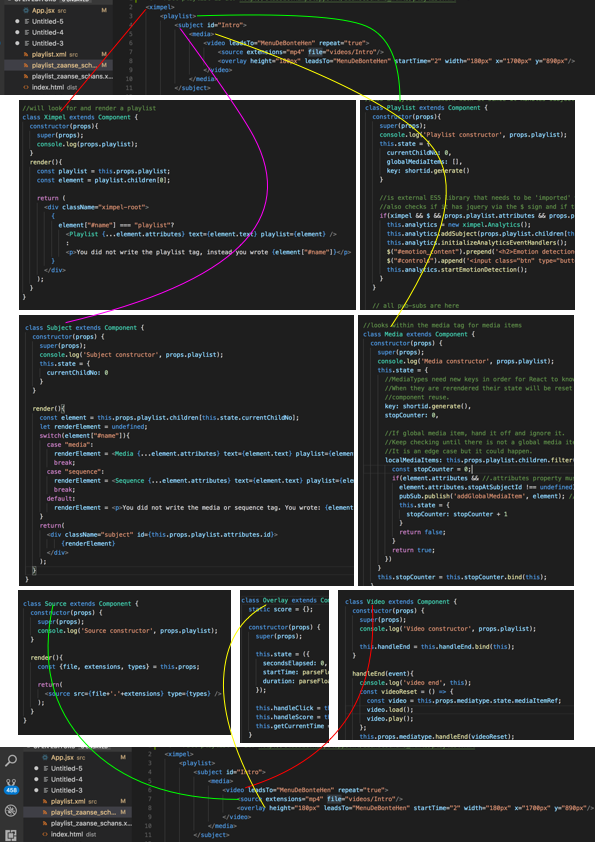
\includegraphics[width=\paperwidth,height=\paperheight]{images/architecture_playlist_to_component_mapping.png}}
%   }
% \caption{test}
% \label{images:architecture_playlist_to_component_mapping}
% \end{figure}
% \newpage


\begin{figure}
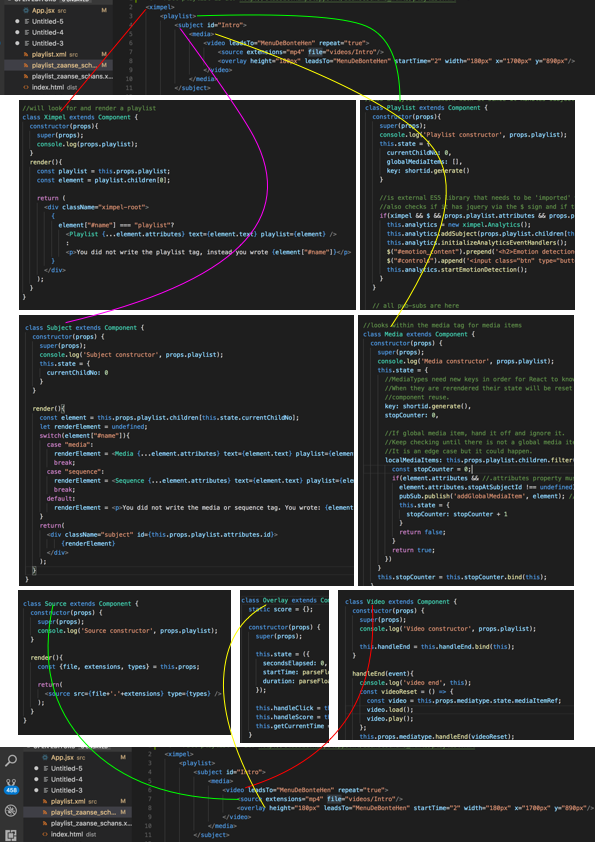
\includegraphics[scale=0.8, center]{images/architecture_playlist_to_component_mapping.pdf} % quotation marks make sure file name does not display
\caption{An example of how a XIMPEL playlist maps onto React components.}
\label{images:architecture_playlist_to_component_mapping}
\end{figure}

\subsection{XIMPEL tags mapped to React component and the link to compiler construction}
To start off this section: consider the following excerpt of the De Zaanse Schans playlist (see code section \ref{playlist:ximpel_zaanse_schans}).

\begin{lstlisting}[language=XML, caption=An excerpt of the De Zaanse Schans playlist., label=playlist:ximpel_zaanse_schans]
<ximpel>
    <playlist>
        <subject id="MenuDeBonteHen">
            <media>
                <video repeat="true">
                    <source extensions="mp4" file="videos/MenuDeBonteHen"/>
                    <overlay height="100px" leadsTo="WalkToHetJongeSchaap" width="350px" x="200px" y="970px"/>
                    <overlay height="100px" leadsTo="QuizBonteHenIntro" width="350px" x="800px" y="970px"/>
                    <overlay height="100px" leadsTo="TourOfMolenDeBonteHen" width="350px" x="1470px" y="970px"/>
                </video>
            </media>
        </subject>
    </playlist>
</ximpel>
\end{lstlisting}

Every tag here as its own React component. The `<ximpel>` tag has the `Ximpel` component, the `<playlist>` tag has the `Playlist` component and so on. 

This design makes it possible to devise rules for every component, just like it is possible to devise rules for every context free grammar when parsing a programming language. Since a XIMPEL playlist is a declarative language, borrowing conceptual ideas from syntax analysis in compiler construction may prove to be useful for describing XIMPEL's architecture.

A context free grammar (CFG) has four elements to it. A set of non-terminals, a set of terminals, a set of production rules and a starting symbol. Of relevance here are the ideas of: non-terminals, terminals and production rules. Knowing which are which tells more about the architecture. These terms will not be used in a strict sense, but the essence of these ideas will remain. When I clearly deviate from the strictness of one of these ideas it will be written in advance. The idea of production rules will be renamed to component rules since the rules of what every XML tag should do is encoded in the React component that maps to it and strictly speaking they are not production rules (though they have some similarities).

The terminals are the easiest to understand: the media items displayed on the web page are the terminals, such as a video element or audio element. These terminal symbols are not strictly terminals in the CFG sense since they can nest elements as overlays and supporting elements (e.g. `<source>` for the `<video>` tag). They are terminating symbols in the sense that the endless nesting stops and a media item will be displayed. Other terminating symbols are: `<source>` (as a part of `<video>`) and `<overlay>` (as a part of any media type).

The non-terminating symbols are: `<ximpel>`, `<playlist>`, `<subject>`, `<media>` and `<sequence>`. Writing a playlist with only these tags will yield in a meaningless playlist.

\subsection{Component Rules}
The component rules are written per React component in the source code. For architectural purposes, I will present the rules per component, but they may not be fully comprehensive. They will, however, serve for having a strong understanding of the architecture underlying the code base. The rules will be discussed from top to bottom. 

\subsubsection{Ximpel}
The `Ximpel` component checks whether the `<ximpel>` tag has been written. 

It sees if there is a `<playlist>` tag underneath it and will output a warning on the page and not render anything else. 

It does not check if there is one `<ximpel>` tag. 

\subsubsection{Playlist}
This component tracks which subject is being played. 

It also tracks all the global media items (media items that survive a subject switch, i.e. a global media type) and renders them if needed. 

It initializes the logging framework the `enableLogging` attribute is set to ``true''. 

It also has two subscribed methods in the publish-subscribe system that XIMPEL React uses. 

It listens to any component publishing a topic on `leadsToUpdate` and it will update its own state to render a new subject. 

It also listens to when a `Media` or `Sequence` component signifies the topic of `addGlobalMediaItem`, in which case it adds a media item to its own `globalMediaItems` array so the media item is able to survive the subject switch. 

It renders the global media items and the underlying `<subject>` tag. If no `<subject>` tag has been specified it will display an error message on the page.

\subsubsection{Subject}
This component looks for the underlying `<media>` or `<sequence>` tag. If it is not there it will display an error message on the page.

\subsubsection{Media}
This component plays media items in parallel. 

It is able to render a `<sequence>` tag or any media tag. 

It will give an error message if no media type tags or `<sequence>` tags are children.

It counts how many of its children have stopped playing and notifies this to the parent. This notification is intended for the `<sequence>` tag. With it, the `<sequence>` tag knows that it is able to continue playing the next media type or `Media` component. If the parent is a `<subject>` then this notification is not relevant.

Before playing it checks to see if its first media item is a global media item. If it is, it will increment the stop counter since the responsibility of a global media item does not belong to the `Media` component but to the `Playlist` component.

When it renders a media tag, it also renders an element that tracks time for the media item as a parent. As of now this is called `MediaType` but it may also be called `MediaManager` later on. Here is a piece of example code.

\begin{lstlisting}[language=JavaScript, caption=An example of how each media item has a general component to manage itself for time tracking (among other things)., label=javascript:media_type_render]
    <MediaType stopCounter={this.stopCounter} {...element.attributes} playlist={element} key={this.state.key + i} render={mediatype => (
        <Youtube {...element.attributes} mediatype={mediatype} text={element.text} playlist={element} />
    )}/>;
\end{lstlisting}

\subsubsection{Sequence}
This component plays a media item (or `<media>` tag) one at a time and will go to the next one when the duration of its current media item is finished. If a media item has no duration specified in the playlist, this media item will be playing it for an infinite amount of time. A `<media>` tag does not need a duration, it only needs to notify the `Sequence` component that it is done rendering all its children.

It will give an error message if no media type tags or `<media>` tags are children.

It counts which child it is playing and whether it is finished playing.

When it is finished playing it will notify its parent that it stopped. This notification is intended for the `<media>` tag so it knows that this component is done with rendering everything. If the parent is a `<subject>` then this notification is not relevant.

When it renders a media tag, it also renders an element that tracks time for the media item as a parent. As of now this is called `MediaType` but it may also be called `MediaManager` later on. 

\subsubsection{MediaType}
The `MediaType` component is the only component that does not have a direct one to one mapping with the XIMPEL playlist. This component applies to all media types and acts a manager for every media type. All media types have a couple of requirements in common which is why this component was created.

It tracks: duration, the amount of seconds elapsed, whether it has to render itself, it also tracks an inner state of whether it should play and the underlying media type and when a media item needs to start playing.

It is able to get information from the underlying media type regarding the amount of seconds elapsed. This feature is also seen in XIMPEL JS, where it has been argued in the comments that the video and YouTube API are better able to track time than the JavaScript implementation of XIMPEL JS itself.

It notifies the `Media` or `Sequence` component when it stopped playing.

It renders overlays that are children of any media type tags. In the general architecture of XIMPEL React it is a rule that an overlay can only be rendered by a media type.

\subsubsection{Media Types}
Most media types simply render themselves, take in the attributes of what was written in the playlist. `Video`, `Terminal` and (in future work) `YouTube` have more than only a call to a render method.

All media types are able to render overlays and overlays are only allowed to be rendered as children of media types.

The `Video` component also tells `MediaType` when it is done playing itself when it is not on repeat and it gives a reference of itself to `MediaType` in order for `MediaType` to improve time tracking (e.g. when a video is paused there is no time elapsing). The `Youtube` component could be programmed to do these things too, but as of now this has not been done yet.

The `Terminal` component connects to a server that runs a bash shell and communicates via web sockets. Because of this, it is able to handle form submission.

\subsubsection{Overlay}
This component has a static variable called `score` which is an object that tracks all the scores that are put as an attribute in the `<overlay>` tag. 

It tracks its own time, except when `MediaType` passes down a reference of the HTML5 video player. Then the time will be tracked for the overlay.

Other than tracking time it also tracks start time and duration.

It renders itself and has no children.

The most important feature of an overlay is that when it is clicked, it will publish a `leadsToUpdate` to any subscriber willing to listen which is the `Playlist` component, since it will start rendering a new `Subject` component, forcing a rerender of a whole new part of the playlist.

% kun je een force unmount doen?
% je kunt een force unmount doen, dus dit zou eventueel kunnen veranderen.
\subsection{Beyond the component rules}
It is important to know that while these rules describe the components fairly adequately, two things have been left unsaid. Certain edge case behavior has not been discussed and lifecycle management issues that needed to be programmed against. An example of one edge case is that the logging framework is written in ES5 and jQuery. Because of this the `Playlist` component needs to check if jQuery exist and use it in order to attach the facial expression classifier part of the framework to the DOM. An example is key management, which is needed for almost any React component out there. If React needs to use deep diffing into the DOM, then the lifecycle methods will be called at unfortunate moments. This is an issue if a new developer does not understand key management and how it influences the lifecycle methods. Currently it is not a problem anymore, but it used to be.

\subsection{Data flow within XIMPEL React}
The data flow within XIMPEL React tries to follow conventional ReactJS philosophy: try to have a unidirectional data flow as much as possible. Which means data flowing from parent to child. However, sometimes this is not possible. If a child gets a state change earlier which a parent also would need to know, then it in some cases becomes difficult to do so. Conventional React best practice suggests to lift state. However, this has not always seemed to be possible, but furthermore it makes code readability worse.

For child to parent communication I used callbacks or render props (through which I could use callbacks). For great great great ... great grandchild communication to the `Playlist` component I used a publish subscribe library called PubSub.js \cite{pubsubJS}. Some people reading this may ask themselves ``why did you not use the Redux library?`` The answer simply is: it was not needed. I know that a lot of developers use the flux architecture for solving data flow communication issues, but this is only needed when current data flow communication solutions become unwieldy. This is not the case for XIMPEL React. It may be the case in the future, when the codebase passes 5000 lines or 25000 lines (who can tell?) and then refactoring will be needed.

% Op welke manier passen questions in XIMPEL?
% React als ecosysteem? Te doen?
% Maintainability
% Is de React codebase zinvol? Voor? Tegen? Eventuele uitbreidingen?
\section{Conclusion}
So who is hungry? It is about time to assess whether porting XIMPEL in React provides a free lunch! The assessment works as follows. First, unexpected advantages and disadvantages will be taken into consideration. Then, the expected advantages will be evaluated by asking: to what extent were positive development factors in reality?

\subsection{Unexpected advantages and disadvantages}
The biggest downside of React was not the library itself but the learning curve of it. The fine-grained understanding over the lifecycle and key management has produced hundreds of lines of code that were ultimitaly unecessary and have been refactored out. Without this fine-grained understanding, more control over the DOM would be nice, as well as knowing when the lifecycle methods would be triggered. Fortunately, it was a learning curve issue and nothing else. 

The pro's of the React and Webpack combination were plentiful. One advantage mentioned earlier is that React components map really well on XML elements of the XIMPEL playlist. Since the component abstraction rarely breaks, it is fairly easy to reason what each XML element is responsible for regarding which React component. 

Another advantage that came to light later on was the lack of DOM manipulation needed. React does this. Normally, a developer needs to be concerned about: state, rendering HTML (most likely with jQuery) and when to render the HTML. With ReactJS the only concerns are having the right state and rendering it, which simplifies reasoning about the whole application since the question of when to render HTML is gone.

One future advantage is when XIMPEL or concepts like XIMPEL will be used for mobile applications. React Native shares a lot of similar code with ReactJS and to port it over to mobile should be possible. One interesting caveat is that mobile applications need to be reviewed by their respective app stores. However, a playlist that is sent over the server does not need to be reviewed. So a technique to extend an app is to create one's own custom declarative language and load it in as a playlist, like XIMPEL does. A related advantage is that it is almost within reach to create mobile apps with XIMPEL. The framework has to be adapted to React Native, which has a lot of code in common with ReactJS, in general.

% https://github.com/Leonidas-from-XIV/node-xml2js
\subsection{Evaluating the expected advantages}
The first pro is that a lot of parsing logic could be done with React and Webpack. This is true, but interestingly enough, not by transforming the XIMPEL playlist to a language that is completely compliant with JSX. The XML loader of webpack had (in hindsight) a strong XML parser that was a good library to use \cite{node_xml2js}. This parser created a workable in-memory configuration object.

Which brings us to the second pro. The virtual DOM would replace the in-memory configuration code. So there is no need to write in-memory configuration code. While it has been tried to use the virtual DOM to replace the in-memory configuration code, this has been tedious -- this has been done in the second attempt. As stated in the previous paragraph, the actual parsed XML tags were used, which provided the in-memory configuration that was needed -- this has been done in the third attempt.

% https://reactjs.org/blog/2016/01/12/discontinuing-ie8-support.html
% https://reactjs.org/docs/javascript-environment-requirements.html
The third pro is that cross-browser support is managed by the maintainers of the ReactJS framework. This is unfortunately not entirely true since the logging framework has not been ported to React. ReactJS itself support Internet Explorer 9 and higher through the use of some polyfills. It used to support Internet Explorer 8, but it has discontinued support since the beginning of 2016 \cite{react_discontuining_ie8}.

The final advantage was a didactic one. Students who want to extend XIMPEL React need to learn a thing or two about ReactJS. This in turn leads them to learn some computer science concepts. It is hard to assess this potential advantage, but since I needed to brush up on my ReactJS skills, I can review which programming concepts I have gained a better understanding of. These are: lifecycle methods, diffing, performance between a virtual DOM and actual DOM, the DOM itself, some basics of functional programming (I did not follow the course in my bachelor degree), the render and state cycle, the lifecycle of a component (it is reminiscent of the iOS framework Cocoa and Cocoa Touch which also has lifecycle methods) and key management (unique identifiers). It could be argued that some of these concepts are also computer science concepts. Regardless of whether it is true, students who want to extend or play with the core of XIMPEL will learn a lot about web development.

\subsection{Concluding the evaluation}
In summarized fashion, the advantages of ReactJS are: no DOM manipulation, XML attributes easily included as props (thanks to a combination of React and the XML parser), strong one to one mapping to the XIMPEL playlist, cross-browser support, strong error reporting, a strong ecosystem, and porting options to mobile and tablet. The strong one to one mapping to the XIMPEL playlist has been very useful for development. Focusing on solely one tag and writing out the component rules for that tag is helpful. Regarding the props of ReactJS, it has not been needed to attach the XML attributes to anything, unlike in XIMPEL JS. The ecosystem of React is perhaps its strongest advantage since it offered easy discoverability for libraries that saved a lot of time, such as the XML parsing library or the ability to write ES6 with Babel. This means: less code to write, an architecture that is fairly easy to reason about, maintainability out of the box and rapid software development options on other platforms. This is a lot. A speculative advantage is that ReactJS might segment its position as a best practice for the web. 

The only downside is that people need to learn it and become proficient in it. Fortunately, the learning curve should not be that high since XIMPEL React only uses ReactJS its core library and DOM library. It does not use other popular libraries from the React ecosystem that invite a learning overhead (e.g. Redux). Hence, the downside is relatively contained compared to other React ports.

Does this mean that we should abandon ship and stop the development of XIMPEL JS? Compared to the development time of XIMPEL React, the creation of XIMPEL JS has also been realized relatively quickly. While I do not have data on the matter, my guess would be that it has been made within 336 to 672 hours of development time. Bruins developed XIMPEL JS for his master thesis, and had (officially) 1004 hours time for the whole thesis. The point is: that is still relatively quick. 

As of now, XIMPEL React is a subset of XIMPEL JS and has a couple of different design decisions. Therefore, no version of the framework replaces the other. The design decisions of XIMPEL React easily shows whether the design decisions taken were a good idea. XIMPEL React has no: pause and resume functionality, quiz tags, constant dimensions (i.e. 1920 x 1080). Some media items have rudimentary video and audio time scrubbing. Preliminary results show that: quizzes can still be modeled; even quizzes with feedback and not having constant dimensions has consequences of the positioning system in such a way that it is identical to positioning web elements. 

To close this chapter, this exploration is a final exploration in disguise. Since it had three attempts, only the first attempt was the actual third exploration which is now in appendix \ref{chap:exploration3_appendix_part1}. The second and third attempt can be seen as the seventh exploration respectively. When I ported XIMPEL to React successfully in my second attempt and fine-tuned it in my third attempt, the first rough draft of everything (including this chapter) was already written and everything else was already programmed. So other than an assessment to see whether XIMPEL could be ported to React, this port also showcases a particular vision of XIMPEL. The other explorations serve as puzzle pieces of programming and design explorations and they serve as an inspiration for this implementation of XIMPEL React.